\cut{
  - HMM
  - Hierarchical Maximum entropy
  - Hierarchical Support Vector Machine
  each: give the formula -> intuition, examples to show where we work well
  and where we work badly
}


\section{Statistical Models}\label{sec:stats}

\cut{As discussed in Section \ref{sec:algo}, our new algorithm considers all possible
token sequences rather than the only one defined by a fixed set of
regular expressions. Therefore a seqset that contains all legal token
sequences is constructed for each chunk. But, the histogram-computing
module afterwards requires one single token sequence from each chunk
and uses these tokens as the basic units to extract structure
information.}

A key component of the format inference algorithm described in the 
previous section is a selection of the best token sequence from
each \seqset{}.  To prioritize sequences, the algorithm 
assigns probabilities using a statistical token model.  This
section describes three such models that we have experimented with.


%% to solving the token ambiguity problem is to select the best
%% token sequence from the many possible sequences represented by a
%% \seqset{}. Machine learning techniques,
%% which build probabilistic models from labeled training data,
%% ar%% e applicable to the token ambiguity problem for the following reasons.

%% \begin{itemize}
%% %\item Training corpus can be construct efficiently. Instead of
%% %assigning tags token by token, system designers
%% %only need to write the correct descriptions by hand for the data
%% %formats selected as training sources. We've devised a tagging tool to
%% %label the tokens automatically given the data source and the
%% %corresponding description;
%% \item Large amounts of ad hoc data exist from which we can learn token models.
%% \item The \pads{} infrastructure allows us to label large amounts of training data quickly.
%% \item Common tokens with distinctive features appear frequently in
%%   multiple sources.  For example, URLs usually start with  ``\texttt{http://}'',
%%   and items that look like times, such as ``\texttt{04:12:59},'' make
%%   certain strings more likely to be parts of dates, such as
%%   ``{\tt March}''.  This observation means that we can build a
%%   model of various tokens based on training data and then apply those
%%   models to new data sources.
%% \item We can use efficient procedures from machine learning, such as
%%   the Viterbi algorithm~\cite{rabiner89:hmm}, to find the most likely token
%%   sequences from learned models.
%% \end{itemize}
\cut{
In the training corpus, examples are chunks annotated with token
sequences, each token with its associated substring. A statistical
model is trained ahead of time. In the structure discovery phase of
\learnpads{}, the goal is to label the chunks with token sequences.
}

%% Many different machine learning algorithms
%% exist~\cite{Seymore99learninghidden,Pinto+:texttables,borkar+:text-segmentation,rabiner89:hmm}.
%% We have experimented with three different techniques for 
%% building probabilistic models of tokens, which
%% we describe in the following subsections.

\paragraph*{Character-by-character Hidden Markov Model (HMM)}\label{subsec:hmm}

The first model we investigate is the classic first-order,
character-by-character Hidden Markov Model (HMM)~\cite{rabiner89:hmm}.
An HMM is a statistical model that includes one set of
states whose values we can observe and a second set whose values are
{\em hidden} and we wish to infer.  The hidden states determine, with
some probability, the values of the observable states.  In our case,
we can observe the sequence of characters in the input string and wish
to infer the token that is associated with each character.  
The model assumes the probability that we see a particular character 
depends upon its associated token and moreover, since the
HMM is first-order, the probability of observing a
particular token depends upon the previous token but no other
earlier tokens.  The picture below illustrates the process of
generating the character sequence ``2.2.13-4'' from a token
sequence.  Hidden HMM states are white and observables are shaded.  
Notice particularly that the adjacent digits ``1'' and ``3'' are 
generated from two consecutive instances of the token {\tt int},
when in a true token sequence, both characters are generated from 
a single {\tt int} token.  A postpass will clean this up, but such 
situations are dealt with more effectively by the HMEMs described in
the following subsection.

%% %% , represents the true state of a system as a
%% %% finite collection of ``hidden states.''  The states are hidden because
%% %% we cannot directly detect which state the system is in, and instead
%% %% must try to infer the state from observing what it emits.  
%% %% Furthermore, the hidden 
%% %% state is allowed to change upon each observation.  In our setting,
%% %% each token type corresponds to a hidden state, and each character to
%% %% an observation.
%% \figref{fig:hmm} shows a first-order HMM representation of a substring
%% from {\tt yum.txt}.  
%% The qualifier ``first-order'' indicates that the
%% current state depends only upon the previous state. 
%% Each observation, indicated as a shaded node, is a single character. 
%% Each hidden state, indicated as a white node, 
%% is the name of the token that describes the
%% corresponding observable character. We use arrows to denote
%% both the dependence among the hidden states and the emission of
%% observations by the hidden states.
%% We call the hidden state in the character-by-character HMM 
%% a {\em partial token} because the corresponding character is often
%% only a part of a full token.


%\begin{figure}[th]
\begin{center}
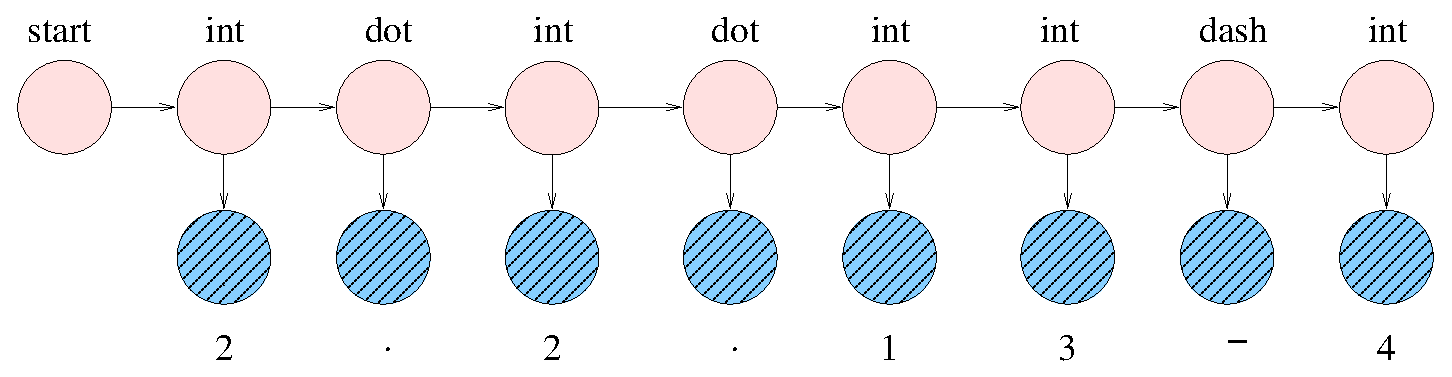
\epsfig{file=hmm.eps, width=0.7\columnwidth}
\end{center}
%\caption{HMM of a partial token sequence from string ``2.2.13-4''}\label{fig:hmm}
%\end{figure}

Finally, since our training data is limited, we employ one further
approximation in our model. Instead of modelling every individual
character separately, we classify characters using a set of boolean features
including features for whether the character is (a) a digit, (b) an
upper-case alphabetic letter, (c) white space, or (d) a particular
punctuation character such as a period.  We call the feature vectors
involving (a)-(d) {\em observations}.

%
% To avoid bias toward certain characters, we use
% a fixed-length \textit{feature vector} instead of the character itself
% as the observation. Each feature vector contains a
% fixed number of boolean features about a single character, such as
%Note that we use character
%feature vectors as opposed to plain characters as observations,
%because in many cases, we don't want the model biased towards
%certain characters. For example, if most {\em time} tokens in the
%training corpus are drawn from the software running in a certain
%range of time, some digits will never appear to be the first
%character in {\em time}. To avoid this bias, we define a mapping
%from characters to fix-length vectors and use these vectors to
%represent features of characters. Examples of features are:
%% \begin{itemize}
%% \item is a numeric digit
%% \item is an upper-case alphabetic letter
%% \item is white space
%% \item is a special punctuation, ``{\tt .}''
%% \item is a punctuation other than ``{\tt .}'', ``{\tt
%% ,}'', ``{\tt ?}'', ``{\tt /}'', ``{\tt $\backslash$}" and ``{\tt :}''
%% \end{itemize}

Let $\mathbf{T}_i$ denote the $i^{th}$ hidden state; its value ranges over
the set of all token names.
Let $\mathbf{C}_i$ denote the observation emitted by hidden state $\mathbf{T}_i$.
Three parameters determine the model:
the transition matrix $\mathbf{P}(T_i|T_{i-1})$,
the sensor matrix $\mathbf{P}(C_i|T_i)$ and the initial
probabilities $\mathbf{P}(T_i|begin)$. 
We compute these parameters from the training data as follows:

\begin{eqnarray}
\mathbf{P}(T_i|T_{i-1}) & = & \frac{\textrm{occurrences where}~ T_i\textrm{
follows}~ T_{i-1}}{\textrm{occurrences of}~ T_{i-1}} \label{eqn:1}\\
\mathbf{P}(C_i|T_i) & = & \frac{\textrm{occurrences of}~ C_i \textrm{
annotated with}~ T_i}{\textrm{occurrences of}~ T_i} \\
\mathbf{P}(T_1|begin) & = & \frac{\textrm{occurrences of}~ T_1~ \textrm{being first token}}
{\textrm{number of training chunks}} \label{eqn:2}
\end{eqnarray}

Given these parameters and a fixed input, we want to find the token
sequence with the highest probability, \ie{}, from the input sequence 
$C_1, C_2, ..., C_n$, we want to find the token sequence 
$T_1, T_2, ..., T_n$ 
that maximizes the conditional probability
$\mathbf{P}(T_1, T_2, ..., T_n|C_1, C_2, ..., C_n)$.
This probability is defined as usual:

\begin{eqnarray}
\mathbf{P}(T_1, T_2, ..., T_n|C_1, C_2, ..., C_n) & \propto & \mathbf{P}(T_1, T_2, ..., T_n, C_1, C_2, ..., C_n) \nonumber \\
& = & \mathbf{P}(T_1|begin) \cdot
\prod_{i=2}^{n}{\mathbf{P}(T_i|T_{i-1})}
\end{eqnarray}

\cut{
To guarantee linear-time efficiency, the Viterbi algorithm to compute
the most likely sequence is employed. In our problem, not every
combination of tokens as a sequence is a legal parse given a chunk. So
the Viterbi algorithm has to be modified so that the most likely sequence
returned by the algorithm is the one among all possible parses. If we
consider this requirement as a constraint to the output, in fact, a
variety of modified Viterbi algorithms are deployed in the
\learnpads{} system to satisfy corresponding constraints at different
places. Due to the space limitation, we'll show only one of them in
Subsection \ref{subsec:hmem}.
}
To calculate the highest probability token sequence from this
model, we run a slightly modified variant of the Viterbi 
algorithm over the \seqset.
%to ensure that the most probable token sequence returned forms a legal
%parse of the data chunk. 
%{\bf Is the above formula an instance of
%  the viterbi algorithm?  If so, we should say so. If not, this last
%  sentence needs to be linked in better.}

Because the character-by-character HMM is first-order and employs only 
single character features, it cannot capture complex features
in the data such as  
a substring ``{\tt http://}'' which indicates a strong likelihood 
of being part of a URL.
%This HMM assumes every partial token is only dependent on its previous
%partial token. So the first-order Markov Model is a simple model that
%is unable to catch complicated features. 
One obvious solution is increasing the order of the HMM.  However, since
the token length is variable in our application, it is not clear what
the order should be.  In addition, increasing the order also increases
the complexity exponentially.  Instead, in the next sections, we pursue
two hybrid methods that incorporate existing classification techniques
into the HMM framework.

\paragraph*{Hierarchical Maximum Entropy Model (HMEM)}\label{subsec:hmem}

The character-by-character HMM extracts a set of features from each character
to create an observation and then runs a standard HMM over these observations.
In contrast, the Hierarchical Maximum Entropy Model (HMEM), which we
will explore next, extracts a set of features from each substring, uses
the Maximum Entropy (ME) procedure~\cite{Berger96:ME,megaweb}
to produce an observation and runs a standard HMM over these new kinds
of observations.  
Using the sequence ``2.2.13-4'' as our example again, the corresponding
HMEM may be drawn as follows:

%\begin{figure}[th]
\begin{center}
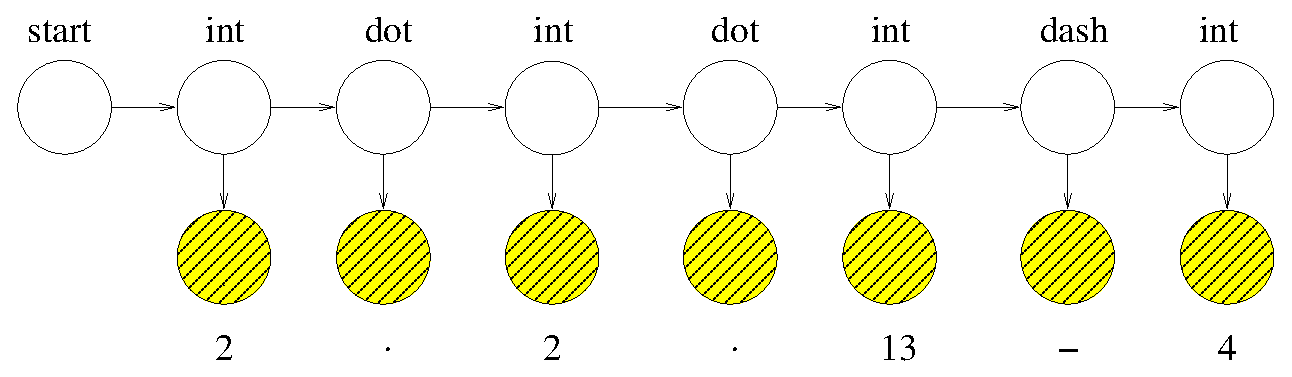
\epsfig{file=hmem.eps, width=0.6\columnwidth}
\end{center}
%\caption{HMEM of a token sequence from string ``2.2.13-4''}\label{fig:hmem}
%\end{figure}

%\figref{fig:hmem} shows an example of HMEM.
%We can see that the graph of Hierarchical Maximum Entropy Model is
%similar to the one in Subsection \ref{subsec:hmm}, because the upper
%level of this hierarchical model is still an HMM. 
%The main difference between HMEM and HMM is
%that an observations is not a single character feature vector, 
%but a substring corresponding to a whole token.
%As such, there is no need to concatenate consecutive partial tokens
%to form a whole token as in the case of HMM.

Formally, let $\mathbf{T}_i$ be the $i^{th}$ hidden state or token in the
sequence (denoted by a white node in picture above) and
let $\mathbf{S}_i$ be the substring annotated by $\mathbf{T}_i$. 
Suppose the number of tokens in the chunk is $l$; then the
target probability is as follows.

\begin{equation}
\mathbf{P}(T_1, T_2, ..., T_n|S_1, S_2, ..., S_l)  \propto
\mathbf{P}(T_1|begin) \cdot \prod_{i=2}^{l}{\mathbf{P}(T_i|T_{i-1})}
\cdot \prod_{i=1}^{l}\mathbf{P}(S_i|T_i)
\end{equation}

Equations (\ref{eqn:1}) and (\ref{eqn:2}) allow us to calculate
the transition matrix and the initial probability.
%Then the question comes to how to estimate $\mathbf{P}(S_i|T_i)$.
We can compute $\mathbf{P}(S_i|T_i)$ using Bayes Rule,
\begin{eqnarray} \label{eqn:bayes}
\mathbf{P}(S_i|T_i) = \frac{\mathbf{P}(T_i|S_i) \cdot
\mathbf{P}(S_i)}{\mathbf{P}(T_i)}
\end{eqnarray}

Finally, since obtaining accurate estimates of 
$\mathbf{P}(S_i)$ and $\mathbf{P}(T_i)$ appears to require more training
data than we currently have, we have further approximated by simply
using
%Because the training corpus comes from real world applications, 
%the terms $\mathbf{P}(S_i)$ and $\mathbf{P}(T_i)$ in (\ref{eqn:bayes})
%can differ substantially between the training and
%testing data, making them poor parameters for 
%the prediction. To compensate, we use ME 
%to compute 
$\mathbf{P}(T_i|S_i)$ to estimate $\mathbf{P}(S_i|T_i)$.
Estimation of $P(T_i|S_i)$ through the ME procedure involves using
the following features (among others):
(a) total number of characters in the string,
(b) the number of occurrences of certain punctuation characters,
(c) the total number of punctuation characters in the string,
(d) the presence of certain substrings such as ``{\tt am}'', ``{\tt pm}'', 
``{\tt January}'', ``{\tt Jan}'', ``{\tt january}'', and
(e) the presence of digit sequences.
When we substitute $\mathbf{P}(T_i|S_i)$ for
 $\mathbf{P}(S_i|T_i)$ in equation (5), we obtain the following:

\begin{eqnarray}\label{eqn:est-bayes}
\mathbf{P}(T_1, T_2, ..., T_n|S_1, S_2, ..., S_l) \propto
\mathbf{P}(T_1|begin) \cdot \prod_{i=2}^{l}\mathbf{P}(T_i|T_{i-1})
\cdot \prod_{i=1}^{l}\mathbf{P}(T_i|S_i)
\end{eqnarray}

Finally, notice that in equation (\ref{eqn:est-bayes}), the number of tokens
in a sequence will determine the number of terms in the product. 
Consequently, a sequence with more tokens will produce
more terms, which our experiments have shown produces a significant 
bias towards shorter token sequences.  
%% Suppose we are
%% given the data chunk {\tt s} and the probabilities in \figref{fig:ME},
%% \begin{figure}[t]
%% \begin{centercode}
%% s  = ``Dec 10 04:07:51 Updated''
%% P( date | ``Dec 10'' ) = 0.8
%% P( white | `` `` ) = 1.0
%% P( time | ``04:07:51'' ) = 0.9
%% P( word | ``Updated'') = 0.8
%% P( white | others ) = 0.7
%% P( others | white ) = 0.8
%% \end{centercode}
%% \caption{Probability assumptions of a simple example}\label{fig:ME}
%% \end{figure}
%% %
%% where {\tt others} represents tokens other than white space and
%% punctuation. With these assumptions, we compute the conditional probability
%% \[\mathbf{P}(\mbox{date white time white word}~ | \mbox{``Dec 10 04:07:51 Updated''}) = 0.181 \]
%% If we had a token {\tt message} that can parse the entire chunk,
%% the algorithm would select the shorter token sequence {\tt message}
%% even if the probability of the token {\tt message} given the entire
%% string is small, \eg{} 0.3.  
To avoid such bias, we modify
Equation (\ref{eqn:est-bayes}) to use the average log likelihood.

\begin{eqnarray}
&& \log \mathbf{P}(T_1, T_2, ..., T_n|S_1, S_2, ..., S_l) \nonumber \\ 
& \propto & \frac{\log \mathbf{P}(T_1|begin) +
\sum_{i=2}^{l}\log \mathbf{P}(T_i|T_{i-1}) + 
\sum_{i=1}^{l}\log \mathbf{P}(T_i|S_i)}{l}\label{eqn:mod-viterbi}
\end{eqnarray}
\noindent
Using average log likelihood 
guarantees that the algorithm will not select shorter token sequences
unless the average value of all conditional
probabilities $\mathbf{P}(T_i|S_i)$ exceeds a threshold.

To find the highest probability sequence for a chunk under this model,
we implemented a modified Viterbi algorithm
that takes into account the number of tokens in the sequence.
In what follows,
let the number of characters in the chunk be $n$ and the number 
of tokens be $l$.  Let $C_i$ be the character at position $i$, and 
$PT_i$ be the partial token that emits the character $C_i$. 
%Note that if position $i$ is a non-start vertex in the \seqset{}, 
%there must be a token whose ending position is
%$i$ in a legal token sequence. 
Then
$\mathbf{P}(PT_1, PT_2, ..., PT_i|C_1, C_2, ..., C_i, k)$ is the
probability of a partial token sequence $PT_1, PT_2, ..., PT_i$
conditioned on a substring of characters $C_1, C_2, ..., C_i$,
collectively emitted by a sequence of $k$ tokens.
Now, let $T_i$ be a token
that ends at position $i$ and let $S_i$ be the corresponding substring. 
The probability of the most likely partial token sequence up to position 
$i$ is
\begin{eqnarray} 
&&\displaystyle{\max_{PT_1, ..., PT_i}}\log\mathbf{P}(PT_1, PT_2, ..., PT_i,
PT_{i+1}|C_1, C_2, ..., C_{i+1}, k+1) \propto \nonumber \\
&& \nonumber \\
&&\left\{
  \begin{array}{ll}
    \log \mathbf{P}(S_{i+1}|T_{i+1}) + 
    \displaystyle{\max_{T_{i+1-\delta}}}(\log\mathbf{P}(T_{i+1}|T_{i+1-\delta}) + \\
    \qquad \displaystyle{\max_{PT_1, ..., PT_{i-1}}}\log\mathbf{P}(PT_1, ..., PT_i|C_1, ..., C_i, k)), 
& \\ 
  \qquad \hbox{if $i+1$ is the end of an edge in \seqset{},
  $\delta$ is the length of token $T_{i+1}$;} \\\\
    \displaystyle{\max_{PT1, ..., PT_i}}\log\mathbf{P}(PT_1, ..., PT_i|C1, ...,
  C_i, k+1) \\
\qquad \hbox{otherwise.}
  \end{array}
\right. \label{eqn-forward}
\end{eqnarray}

The left-hand-side of (\ref{eqn-forward}), known as a {\em forward message},
contains the token sequence up to a position $i$ in the chunk as well as the 
lengths of
the tokens. 
%At each position $i$, the forward messages store not only token
%sequences ending with different tokens, but also the sequences of different
%lengths. 
At the last position $n$, we compute $l$ from 

\begin{equation}
\max_{l}~ \log \frac{\mathbf{P}(TP_1, TP_2, ...,
TP_n|C_1, C_2, ..., C_n,l)}{l}
\end{equation}
\noindent
and select the last token in the most likely token
sequences. After tracing backwards through the chain of messages,
we obtain the most likely token sequences. The modified Viterbi
algorithm is linear to the number of characters $n$ in the chunk.

%When testing the accuracy of HMEM, we found an empirical
%disadvantage of this model. Training data are collected from their
%original sources without many extra efforts except running the
%automatic token tagging tool. In order to make sure there're
%sufficient data to train the models, every record is directly put into
%the training corpus. But on the other hand, much more work needs to be
%done to find a perfect training corpus that can reflect the true
%distribution of tokens needs. For example, in the training data,
%suppose we have only 1\% {\tt url} tokens, it doesn't mean the
%chance {\tt url} tokens appear in the testing data source is also
%small. 
We saw there were some problems with the basic HMM model that motivated
the use of the HMEM model.  What further problems plague the HMEMs?
The most worrisome problem is that the HMEM is a
generative model that simulates the procedure of generating the data, and
estimates the target conditional probability by a joint
probability. Therefore, it is biased towards tokens with more
occurrences in the training data.  In practice, we found that
when particular tokens appear infrequently in our training data,
the algorithm would never identify them, even when they had
clear distinguishing features. 
%For instance, when there are not enough
%{\tt hostname} tokens in the training data, HMEM cannot identify {\tt
%hostname} tokens effectively and confuses them with {\tt id}
%tokens. 
These difficulties motivated us to explore the effectiveness of Hierarchical
Support Vector Machines (HSVM), which use a discriminative model as 
opposed to a generative one.

\subsection{Hierarchical Support Vector Machines (HSVM)}\label{subsec:hsvm}

An HSVM is exactly the same as an HMEM except it uses 
a Support Vector Machine (SVM) \cite{CC01a} as opposed to Maximum Entropy
to classify tokens. 
Basically, an SVM measures the target conditional probability 
$\mathbf{P}(T_i|S_i)$ 
by generating hyperplanes that divide the feature vector space according to the
positions of training data points. The hyperplanes are positioned so that the
data points (feature vectors in our case) are separated into classes with
the maximum margin between any two classes. The data points that lie on
the margins (or boundaries) of each class are called {\em support vectors}. 

%Though HSVMs can is that they
%effective in detecting less frequently occurring tokens. However, the time
%complexity of SVM is roughly proportional to the number of support
%vectors produced in the training step. Our system generally requires a
%large number of support vectors and thus HSVMs are usually more
%computationally expensive than HMEMs.
